\subsection{GenI Honeynet}
Bei einem GenI Honeynet wird das gesamte Netz durch eine Firewall in drei Teile unterteilt. Der erste Teil ist das Produktivnetz indem sich das zentrale Management System befindet. Der zweite Teil ist das Internet, welcher das Zugangsmedium des Angreifers darstellt. Der dritte und letzte Teil ist das Honeynet\cite{WebGenI.2006b}. 

GenI Honeynets gelten als die ersten richtigen High-Interactive Honeypots, da sie weit mehr Informationen als normale Honeypot, und unbekannte Angriffe aufzeichnen können\cite{spitzner.2002a}.

Der Prozess der Datensammlung beginnt bereits mit passieren der Firewall. Dort können Informationen wie die verwendeten Protokolle, Zeitstempel,IP-Adressen und Ports gesammelt werden. Außerdem wird hier kontrolliert wie oft der Angreifer eine Verbindung eingehen kann (Data Control). Wie viele Versuche zugelassen werden hängt vom Verwendungszweck des Honeynets ab. Der Router zwischen Honeynet und Firewall unterstützt diese auf zwei verschiedene weisen. Zum Einem versteckt er die Firewall vor dem Hacker. Der Angreifer denkt, er greift auf einen produktiven Router zu. Zum Anderen unterstützt er die Firewall in Sachen Zugriffskontrolle. So kann ein Single-Point-of-Failure vermieden werden\cite{grimes.2003a}\cite{WebGenI.2006b}. 

Ein \acf{IDS}-System steht nun noch zwischen dem Angreifer und den Honeypots. Dieses ist meist über einen Switch (oder wie in Abb. \ref{hnet:geni} mit einem Router) mit dem gesamten Honeynet verbunden. Dort werden alle Netzwerkaktivitäten protokolliert und bei bestimmten Angriffsmustern gegebenenfalls ein Alarm ausgelöst\cite{spitzner.2002a}. 

\begin{figure}[ht]
    \centering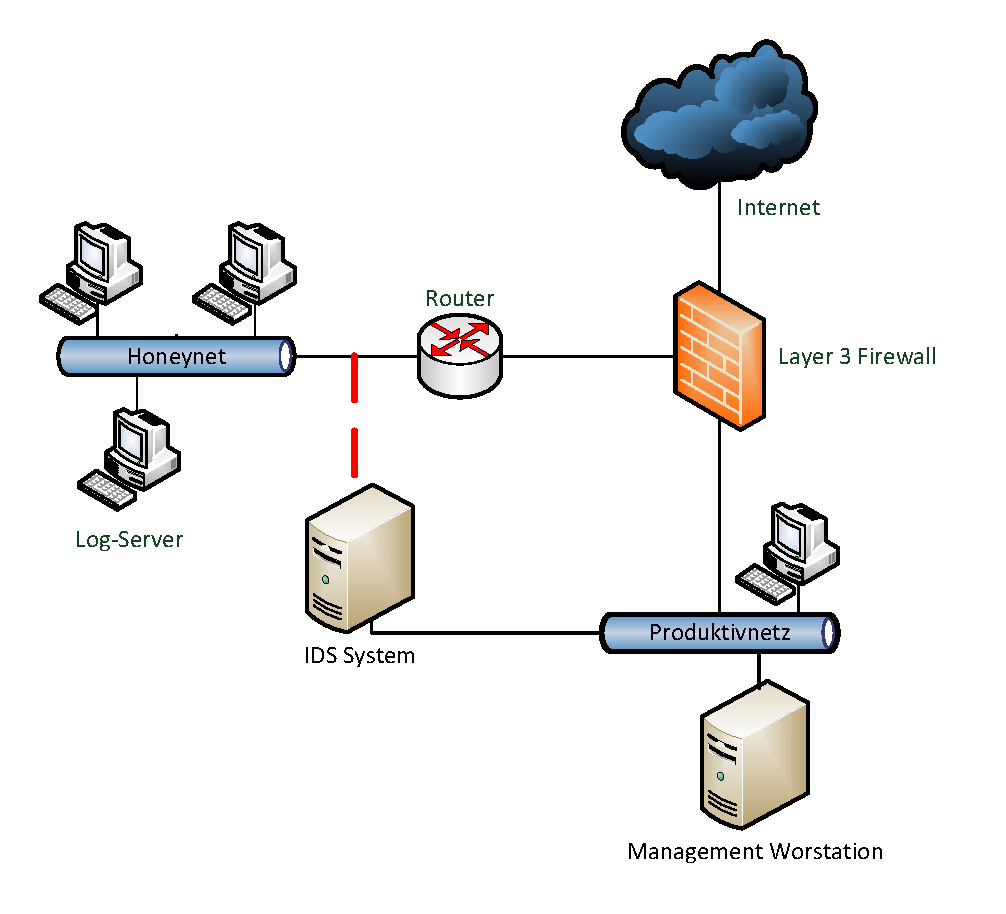
\includegraphics[scale=0.5]{Bilder/GenI.pdf}
  \caption{GenI Honeynet}
  \label{hnet:geni}
\end{figure}

\noindent Die GenI Technologie bietet sich besonders an, um automatisierte oder Anfänger-Hacks zu erkennen. Meist handelt es sich dabei um Ziele, deren Schwachstelle zufällig entdeckt wird, und es dadurch zu einem Angriff kommt. 
Die Architektur ist nicht effektiv für fortgeschrittene Angreifer, oder Hacker, die ein bestimmtes System angreifen wollen. Zum einen sind diese relativ einfach über einen Fingerprint ausfindig zu machen, zum Anderen bestehen sie meist aus einer Standardinstallation eines Betriebssystems, weswegen sie für Angreifer meist uninteressant wirken\cite{spitzner.2002a}.\\

\noindent\textbf{Methoden zur Datenkontrolle}\\
\noindent Die Datenkontrolle eines GenI Honeypots besteht im Grunde aus der Layer 3 Firewall, die das Produktivnetz vom Honeynet trennt. Die Firewall erlaubt jeglichen Zugriff in das Netz, limitiert jedoch die ausgehenden Verbindungen (nicht Pakete). Der Firewall wird vom Administrator eine Grenze für ausgehende Verbindungen mitgeteilt, nach erreichen dieser wird jeder ausgehender Verbindungsversuch geblockt. Je mehr Verbindungen erlaubt sind, desto mehr Freiheiten hat der Hacker seine Aktionen durchzuführen. Um den Schaden zu minimieren die der Hacker verursacht, kann auch eine geringe Grenze gewählt werden. Automatisierte Attacken können so z.B. weiterhin festgestellt werden. Das Honeynet Project empfiehlt hierfür die Linux Firewall IPTables oder als kommerzielle Version FireWall-1 \cite{spitzner.2002a}.\\

\noindent\textbf{Methoden zur Datenaufzeichnung}\\
\noindent Die Datenaufzeichnung eines GenI Honeynets muss, wie zuvor definiert (vgl. Kapitel 3.1), für den Angreifer unsichtbar sein. Die Daten, die gesammelt werden, dürfen nicht lokal auf dem Honeypot gespeichert werden. Um dies zu verwirklichen werden die Daten in verschiedenen Schichten.
Die erste Schicht ist die Logging-Aktivität auf der Firewall. Alle Daten, die in das Honeynet gelange, müssen zunächst durch die Firewall. Dort können zwar keine Informationen wie Tastendrücke oder Packet-Payloads aufgezeichnet werden, jedoch können Protokoll Header, in denen sich Informationen wie Zeitpunkt, Quell- und Zieladresse sowie Quell- und Zielport befinden, ausgelesen und aufgezeichnet werden\cite{spitzner.2002a}. 

Die zweite Schicht ist das IDS-System, welches mit dem Produktivnetz und dem Honeynet jeweils mit einem Interface verbunden ist. Das Interface, dass mit dem Honeynet verbunden ist besitzt keine IP-Adresse. Es gilt als passives Interface (rote Linie in Abb. \ref{hnet:geni}), welches den kompletten Datenverkehr des Honeynets aufzeichnet, jedoch keine Angriffsfläche für den Hacker bietet, da es keine IP-Adresse besitzt. Das zweite Interface erlaubt es dem Administrator im Produktivnetz auf die gesammelten Daten zuzugreifen. Das IDS zeichnet die kompletten Datenpakete mit Payload auf und stellt diese später für eine Datenanalyse zur Verfügung. Die zweite Aufgabe des IDS ist es, eine Warnung bei ungewöhnlichen Aktivitäten zu geben\cite{spitzner.2002a}.

Die dritte Schicht stellen die Honeypots selbst dar. Alle System- und Benutzeraktivitäten sollten lokal und auf dem entfernten Datensammlungsserver aufgezeichnet werden. Selbst wenn der Hacker die lokalen Log-Dateien ändern oder entfernen sollte, die Daten auf dem Datenserver bleiben erhalten. Unter Linux kann ein solcher Server als Remote-Syslog Server in den Logging-Konfigurationen angegeben werden. Mit Windows wird ein Third-Party-Tool notwendig\cite{spitzner.2002a}. Innerhalb des Honeynets soll nicht versucht werden den Log-Server zu verstecken. Entdeckt der Hacker diesen kann dieser höchstens das automatische aufzeichnen deaktivieren. Dies ist jedoch meist das Standardverhalten eines Hackers\cite{spitzner.2002a}. Die Informationen wie der Hacker auf das System kam bleiben jedoch erhalten. Nun wird der Hacker wahrscheinlich versuchen auf den Log-Server zuzugreifen, um dort ihre bereits aufgezeichneten Spuren zu verwischen. Diese Angriffe sind meist komplexer, da ein solcher Log-Server besser geschützt ist. Selbst wenn der Hacker erfolgreich ist, und seine Daten löschen kann, wurde über das IDS trotzdem passiv alle Informationen zum Datenverkehr aufgezeichnet. 
Eine weiter Methode auf dem Honeypot Daten aufzuzeichnen ist über Keystroke-Logger, oder Snapshot Programme, die in regelmäßige Intervallen Screenshots des Honeypots auf einen entfernten Server speichern. Das Honeynet-Project entwickelte hierzu einige Programme. Eine modifizierte Shell kann auf dem Honeypot installiert werden, die die Tastenanschläge mit in die syslog Datei auf dem Log-Server speichert. Oder eine modifizierte Version des TTY Watcher, der Tastenanschläge und Screenshots über eine nicht standardisierte TCP Verbindung an den Log-Server sendet\cite{spitzner.2002a}\cite{grimes.2003a}.

Mit all diesen Möglichkeiten werden die Anforderungen, die in Kapitel 3.1 zum Aufzeichnen der Daten gestellt werden, erfüllt: Netzwerk Aktivitäten, mit der Firewall und dem IDS, der Log-Server zeichnet Anwendungs- und Systemdaten auf, und die Benutzeraktivität kann über eine modifizierte Shell erreicht werden.\\

\noindent\textbf{Probleme der ersten Generation}\\
\noindent Die GenI Honeynet Architektur weißt einige Schwächen auf. Der erste Nachteil besteht in der Datenkontrolle. Die Limitierung der ausgehenden Verbindungen ermöglichen dem Hacker trotzdem andere Systeme außerhalb des Netzes zu attackieren. Das zweite Problem ist Fingerprinting. Hat ein Hacker ein System im Honeynet kompromittiert, so kann dieser testen, ob er nach einer gewissen Anzahl an ausgehenden Verbindungen blockiert wird. Ist dies der Fall, weiß der Hacker das er sich in einem Honeynet befindet. Außerdem kann er über die TTL-Zeit eines TCP-Paketes entdecken, das zwischen dem Produktivnetz und dem Honeynet ein Layer 3 Firewall befindet (diese wird beim passieren um 1 dekrementiert). Das letzte Problem besteht in der Datenaufzeichnung. Syslog-Dateien und Keystrokes werden meist über unverschlüsselte Protokolle versendet, und können so zum Teil als Klartext ausgelesen werden. Benutzt der HAcker nun eine Verschlüsselung, weden diese Daten voreerst nutzlos. Außerdem darf, um diese Informationen zu erhalten, der Hacker syslog nicht deaktivieren\cite{spitzner.2002a}.

All diese Probleme wurden in der zweiten Honeynet Generation aufgegriffen.